\documentclass[10pt,twocolumn,letterpaper]{article}

\usepackage{cvpr}
\usepackage{times}
\usepackage{epsfig}
\usepackage{graphicx}
\usepackage{amsmath}
\usepackage{amssymb}
\usepackage{mathrsfs}
\usepackage{mathtools}
\usepackage{subfigure}
\usepackage{pbox}
\DeclareMathOperator*{\argmin}{arg\,min}
% Include other packages here, before hyperref.

% If you comment hyperref and then uncomment it, you should delete
% egpaper.aux before re-running latex.  (Or just hit 'q' on the first latex
% run, let it finish, and you should be clear).
\usepackage[pagebackref=true,breaklinks=true,letterpaper=true,colorlinks,bookmarks=false]{hyperref}

\newcommand{\deva}[1]{\textcolor{red}{[Deva: #1]}}
\newcommand{\songfan}[1]{\textcolor{blue}{[Songfan: #1]}}

% \cvprfinalcopy % *** Uncomment this line for the final submission

\def\cvprPaperID{1627} % *** Enter the CVPR Paper ID here
\def\httilde{\mbox{\tt\raisebox{-.5ex}{\symbol{126}}}}

% Pages are numbered in submission mode, and unnumbered in camera-ready
\ifcvprfinal\pagestyle{empty}\fi
\begin{document}

%%%%%%%%% TITLE
\title{Supplimentary Material for ``DAG-CNNs for multi-scale recognition''}

\author{First Author\\
Institution1\\
Institution1 address\\
{\tt\small firstauthor@i1.org}
% For a paper whose authors are all at the same institution,
% omit the following lines up until the closing ``}''.
% Additional authors and addresses can be added with ``\and'',
% just like the second author.
% To save space, use either the email address or home page, not both
\and
Second Author\\
Institution2\\
First line of institution2 address\\
{\tt\small secondauthor@i2.org}
}

\maketitle
%\thispagestyle{empty}

%%%%%%%%% ABSTRACT
%\begin{abstract}
%We explore multi-scale convolutional neural nets (CNNs) for image classification. Contemporary approaches extract features from a single output layer. By extracting features from multiple layers, one can simultaneously reason about high, mid, and low-level features during classification. The resulting multi-scale architecture can itself be seen as a feed-forward model that is structured as a directed acyclic graph (DAG). We show that DAG-CNNs are just as fast as chain-structured CNNs in terms of training and testing. In fact, training is easier because multi-scale connections tend to minimize the vanishing gradient problem. We present extensive analysis and results on standard scene benchmarks and show state-of-the-art classification performance on all benchmarks, \ie 55.5\% on SUN397, 76.1\% on MIT67, and 92.4\% on Scene15.
%
%\end{abstract}

%%%%%%%%% BODY TEXT
\section{Full vs. Marginal Features}

In this section, we intend to find out how much we sacrifice when reducing the feature dimension from full response to spatial marginal response of each layer. We conduct this analysis on Caffe-DAG on MIT67. The comparison of full and marginal feature size at each layer is provided in Table.~\ref{table:feat_dim}. The layers of interests are the ones selected by automatic forward-selection as shown in Fig. 7(a) in the main paper. 


\begin{table}[htbp]
\begin{center}
\begin{tabular}{|c|c|c|c|}
\hline
Layer & Response &  Full Feat.& Marginal Feat.\\
\hline
11 & $13\times 13 \times 384$ & 64896 & 384 \\
13 & $13\times 13 \times 384$ & 64896 & 384 \\
15 & $13\times 13 \times 256$ & 43264 & 256 \\
18 & $1\times 1 \times 4096$ & 4096 & 4096 \\
20 & $1\times 1 \times 4096$ & 4096 & 4096 \\

\hline
\end{tabular}
\end{center}
\caption{Feature Dimension for Off-the-shelf Caffe-DAG}
\label{table:feat_dim}
\end{table}

We then train 67-way one-vs-all linear SVM classifiers similar to the experimental setups in the Section 4 for each layer. The classification accuracy is reported in Table.~\ref{table:perf_full}. The performances are identical for Layer-18 and Layer-20 since the \textit{Full-} and \textit{Marginal-feature} are equivalent. Surprisingly, as seen from Table.~\ref{table:perf_full}, the marginal-features always out-perform the full-feature for Layer-11, Layer-13, and Layer-20. This suggests that the full-features is likely to suffer from the ``curse of dimensionality'' given fairly small amount of training data (approximately 5k for MIT67). Thus, choosing marginal over full feature not only improves the classification performance but also reduces feature dimension to manageable ranges. 


\begin{table}[htbp]
\begin{center}
\begin{tabular}{|l|c|c|}
\hline
Layer & Full Feat. & Marginal Feat. \\
\hline
11 & 46.7 & 49.3  \\
13 & 49.0 & 53.8  \\
15 & 52.2 & 54.0  \\
18 & 60.2 & 60.2  \\
20 & 59.6 & 59.6  \\

\hline
\end{tabular}
\end{center}
\caption{Classification Accuary (\%) of Full vs. Marginal Features}
\label{table:perf_full}
\end{table}


\section{Model Fine-tuning}

In this section, we take a deep-dive and consider training our DAG-CNN model in the end-to-end fashion. Firstly, we compare training the Chain and DAG models with softmax loss. We term them \textit{fine-tune} models. Secondly, we use the fine-tune model for feature extraction and analyze the performance using hinge loss. Thirdly, we explore the performance of single- and multi-scale fine-tune models. All the experiments in this section is conducted on MIT67. 


{\bf Chain vs. DAG: } We use the generalized back-propagation algorithm presented in Section 3 to ``fine-tune'' the \textit{DAG} model on MIT67. In comparison, the traditional \textit{Chain} model is also fine-tuned in the same fashion. The data pre-processing step is the same as the one described in Section 4. To prevent over-fitting~\cite{AlexNet}, a dropout layer is inserted after the last FC layer, with the dropout rate of 0.5. The fine-tune chain model is initialized with the pre-trained Caffe model on ImageNet. As we can see from Fig.~\ref{fig:ft_chain}, the final accuracy saturates at 60.7\%. We then initialized our DAG model training with the fine-tuned chain model. As seen from the learning curve shown in Fig.~\ref{fig:ft_dag}, the DAG model stimulates the saturated Chain model and continues to drive the classification performance. Overall, the Caffe-DAG model out-performs the Caffe-Chain, as seen in Table.~\ref{table:ft_models}.


\begin{figure}
\centering
	\subfigure[Chain]{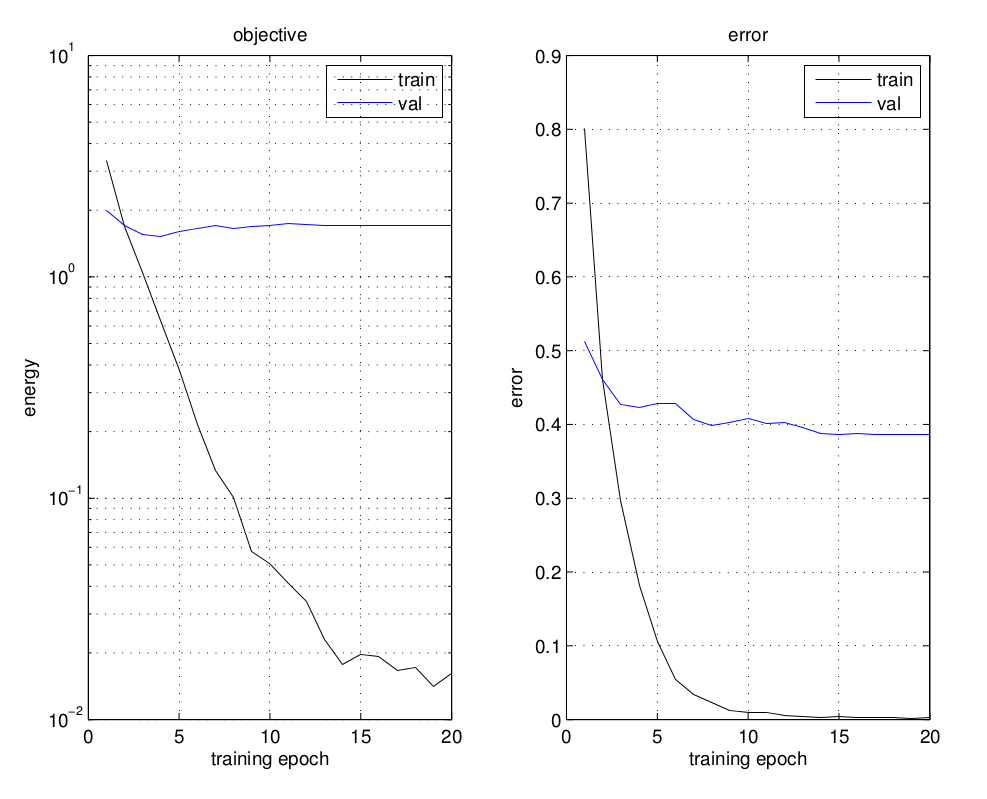
\includegraphics[width=.9\columnwidth]{fig/ft_chain.png}\label{fig:ft_chain}}
	\subfigure[DAG]{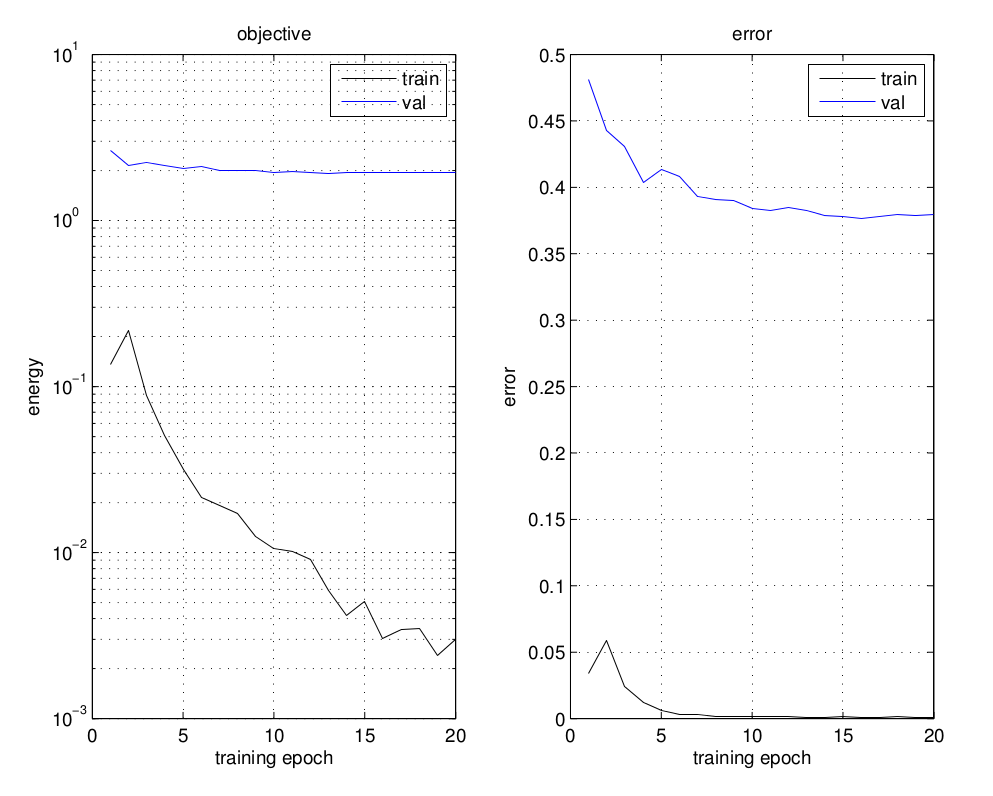
\includegraphics[width=.9\columnwidth]{fig/ft_DAG.png}\label{fig:ft_dag}}

\caption{Fine-tuning Caffe models on MIT67. The left shows the objectives for training and validation set for each epoch; the right shows the corresponding training and validation error.}
\label{fig:ft_curve}
\end{figure}




\begin{table}[htbp]
\begin{center}
\begin{tabular}{|l|c|}
\hline
Structure & Accuracy \\
\hline
Caffe-DAG & 63.5   \\
Caffe-Chain & 60.7   \\

\hline
\end{tabular}
\end{center}
\caption{The comparison of fine-tune Models on MIT67}
\label{table:ft_models}
\end{table}




{\bf Fine-tuning vs. off-the-shelf} 

%We intend to understand how fine-tune model

\begin{table}[htbp]
\begin{center}
\begin{tabular}{|l|c|c|c|c|c|c|}
\hline
& L11 & L13 & L15 & L18 & L20 & multi \\
\hline
off-the-shelf & \textbf{49.3} & \textbf{53.8} & 54.0 & 60.2 & 59.6 & \textbf{64.6} \\
fine-tune Chain   & 48.4 & 51.0 & 55.1 & 61.3 & \textbf{61.7} & 63.5 \\
fine-tune DAG     & 47.8 & 51.6 & \textbf{55.7} & \textbf{61.6} & 61.0 & 64.2	\\
\hline
\end{tabular}
\end{center}
\caption{Single- / Multi-scale accuracy for off-the-shelf and fine-tune Models on MIT67}
\label{table:ft_ots}
\end{table}


{\bf SVM vs. softmax}

\begin{table}[htbp]
\begin{center}
\begin{tabular}{|l|c|c|}
\hline
 & SVM & Softmax \\	
\hline
Single-scale &	61.7 & 60.7 \\
Multi-scale & 63.2 & 63.5   \\

\hline
\end{tabular}
\end{center}
\caption{The comparison of loss function for fine-tune Models on MIT67}
\label{table:loss}
\end{table}


%
%\section{Fine-tune vs. Off-the-shelf}
%
%In this section, we analyze the performance of DAG-CNN trained in the end-to-end fashion on all three datasets. These results is then compared with the off-the-shelf DAG-CNN feature. Concretely, we first train the proposed DAG-CNN model with softmax loss using the algorithm presented in Section 3. We term this \textit{fine-tune} model. On the other hand, the \textit{off-the-shelf} setting is by first concatenating the outputs of the average-pooled features and then trained with hinge loss using Liblinear package~\cite{liblinear}. The results for \textit{off-the-shelf} experimental setup are the reported in the main paper. Here, we provide the results for the \textit{fine-tune} setup as a comparison. 
%
%
%\begin{table}[htbp]
%\begin{center}
%\begin{tabular}{|l|c|c|}
%\hline
%Approach & Off-the-shelf &  Fine-tune\\
%\hline
%Deep19-DAG & \textbf{55.5} &  \\
%Deep19~\cite{veryDeep} & 51.9 &  \\
%Caffe-DAG & 46.6	& \\
%Caffe~\cite{Caffe} & 43.5 &  \\ \hline
%
%\hline
%\end{tabular}
%\end{center}
%\caption{Classification results on SUN397}
%\label{table:SUN397}
%\end{table}
%
%
%
%\begin{table}[htbp]
%\begin{center}
%\begin{tabular}{|l|c|c|}
%\hline
%Approach & Off-the-shelf &  Fine-tune\\
%\hline
%Deep19-DAG & \textbf{76.1} &  \\
%Deep19~\cite{veryDeep} & 70.8 &  \\
%Caffe-DAG & 64.6	& 63.5\\
%Caffe~\cite{Caffe} & 59.5 & 60.7 \\ \hline
%
%\hline
%\end{tabular}
%\end{center}
%\caption{Classification results on MIT67}
%\label{table:MIT67}
%\end{table}
%
%
%
%\begin{table}[htbp]
%\begin{center}
%\begin{tabular}{|l|c|c|}
%\hline
%Approach & Off-the-shelf &  Fine-tune\\
%\hline
%Deep19-DAG & \textbf{92.4} &  \\
%Deep19~\cite{veryDeep} & 90.8 &  \\
%Caffe-DAG & 89.7	& \\
%Caffe~\cite{Caffe} & 86.8 & \\ \hline
%
%\hline
%\end{tabular}
%\end{center}
%\caption{Classification results on Scene15}
%\label{table:Scene15}
%\end{table}



{\small
\bibliographystyle{ieee}
\bibliography{mobib}
}

\end{document}
